\begin{tikzpicture}
	\onslide<1->{
		\node[inner sep=0pt] (A) at (3,0)
		{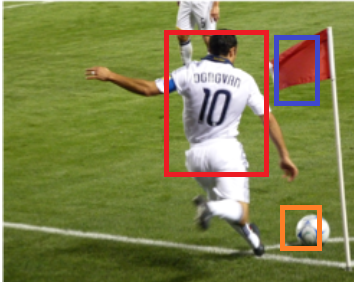
\includegraphics[scale = 0.45]{images/input_2.png}};
		\draw[black, thick, ->]  (4.5,0) --  (5,0);
	}

	\onslide<1->{
		\node [text width = 30mm] at (6,3){Region proposals};
		\node[inner sep=0pt] (A) at (6,0)
		{
\includegraphics[scale = 0.65]{images/region_proposals_2.png}};

		\node [text width = 10mm] at (6.9,-0.8){$h$};
		\node [text width = 10mm] at (6.2,-1.6){$w$};
		
		\node [text width = 10mm] at (7.1,1.9){$h$};
		\node [text width = 10mm] at (6.2,0.9){$w$};
		
		
		\node [text width = 10mm] at (7.1,0.4){$h$};
		\node [text width = 10mm] at (6.2,-0.3){$w$};
	}

	\onslide<3->{
		\tikzstyle{input_neuron}=[circle,draw=red!50,fill=red!10,thick,minimum size=6mm]
		\tikzstyle{hidden_neuron}=[circle,draw=blue!50,fill=cyan!10,thick,minimum size=6mm]
		\tikzstyle{output_neuron}=[circle,draw=green!50,fill=green!10,thick,minimum size=6mm]
		\tikzstyle{cpy_neuron}=[circle,draw=red!50,fill=red!50,thick,minimum size=6mm]
		\tikzstyle{input}=[circle,draw=black!50,fill=black!20,thick,minimum size=6mm]
		\node [text width = 34mm] at (10,3){Feature extraction};
		\node [input_neuron] (neuron51) at (8.5,1.85) {} ;
		\node [input_neuron] (neuron52) at (9.5,1.85)  {};
		\node [input_neuron] (neuron53) at (10.5,1.85)  {};
		\node [input_neuron] (neuron54) at (11.5,1.85)  {};
		\node [text width = 5mm] at (8.7,1.1){$x_1$};
		\node [text width = 5mm] at (9.7,1.1){$x_2$};
		\node [text width = 5mm] at (10.7,1.1){$\dots$};
		\node [text width = 5mm] at (11.7,1.1){$x_d$};
		\draw[red!100,thick,solid,rounded corners=15pt] (8,2.35) rectangle (12,1.35);
	}  
	
	\onslide<2->{
		\node [text width = 50mm] at (14.5,3){Bounding box regression};
		\node[inner sep=0pt] (A) at (13.0,2)
		{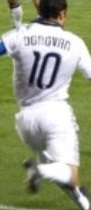
\includegraphics[scale = 0.45]{images/man_corrected.jpg}};
		\node [text width = 10mm] at (14.0,1.7){$h^*$};
		\node [text width = 10mm] at (13.4,1){$w^*$};
		
	}


	\onslide<3->{
		\node [input_neuron] (neuron51) at (8.5,0.35) {} ;
		\node [input_neuron] (neuron52) at (9.5,0.35)  {};
		\node [input_neuron] (neuron53) at (10.5,0.35)  {};
		\node [input_neuron] (neuron54) at (11.5,0.35)  {};
		
		\draw[red!100,thick,solid,rounded corners=15pt] (8,0.85) rectangle (12,-0.15);
	} 
	
	\onslide<2->{
		\node[inner sep=0pt] (A) at (13.0,0.35)
		{
\includegraphics[scale = 0.5]{images/flag_corrected.png}};
		\node [text width = 10mm] at (14.0,0.43){$h^*$};
		\node [text width = 10mm] at (13.4,-0.2){$w^*$};
		
	}
	
	\onslide<3->{
		
		\node [input_neuron] (neuron51) at (8.5,-0.85) {} ;
		\node [input_neuron] (neuron52) at (9.5,-0.85)  {};
		\node [input_neuron] (neuron53) at (10.5,-0.85)  {};
		\node [input_neuron] (neuron54) at (11.5,-0.85)  {};
		
		\draw[red!100,thick,solid,rounded corners=15pt] (8,-1.35) rectangle (12,-0.35);
	} 
	
	\onslide<2->{
		\node[inner sep=0pt] (A) at (13.0,-0.88)
		{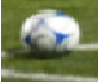
\includegraphics[scale = 0.45]{images/ball_corrected.png}};
		\node [text width = 10mm] at (14.0,-0.8){$h^*$};
		\node [text width = 10mm] at (13.4,-1.35){$w^*$};
	} 
	
	\onslide<3->{
		\draw[black, thick, ->]  (7,-0.85) --  (7.7,-0.85);
		%\draw[black, thick, ->]  (7,-2.15) --  (7.7,-2.15);
		\draw[black, thick, ->]  (7,0.35) --  (7.7,0.35);
		\draw[black, thick, ->]  (7,1.85) --  (7.7,1.85);
		
		\draw[black, thick, ->] (12.1,1.85) --  (12.4,1.85);
		\draw[black, thick, ->] (12.1,0.35) --  (12.4,0.35);
		\draw[black, thick, ->] (12.1,-0.85) --  (12.4,-0.85);
	}
	
	
\end{tikzpicture}